
\documentclass[final]{beamer}

\usepackage{textcomp}
\usepackage{amsmath,amssymb}

\usepackage{subcaption}
\usepackage{color,soul}
\usepackage{url}
\usepackage{hyperref}
\usepackage{adjustbox}
\usepackage{bm}

\usepackage[scale=1.2]{beamerposter} % Use the beamerposter package for laying out the poster

\usetheme{confposter} % Use the confposter theme supplied with this template

\setbeamercolor{block title}{fg=ngreen,bg=white} % Colors of the block titles
\setbeamercolor{block body}{fg=black,bg=white} % Colors of the body of blocks
\setbeamercolor{block alerted title}{fg=white,bg=dblue!70} % Colors of the highlighted block titles
\setbeamercolor{block alerted body}{fg=black,bg=dblue!10} % Colors of the body of highlighted blocks
% Many more colors are available for use in beamerthemeconfposter.sty

%-----------------------------------------------------------
% Define the column widths and overall poster size
% To set effective sepwid, onecolwid and twocolwid values, first choose how many columns you want and how much separation you want between columns
% In this template, the separation width chosen is 0.024 of the paper width and a 4-column layout
% onecolwid should therefore be (1-(# of columns+1)*sepwid)/# of columns e.g. (1-(4+1)*0.024)/4 = 0.22
% Set twocolwid to be (2*onecolwid)+sepwid = 0.464
% Set threecolwid to be (3*onecolwid)+2*sepwid = 0.708

\newlength{\sepwid}
\newlength{\onecolwid}
\newlength{\twocolwid}
\newlength{\threecolwid}
\setlength{\paperwidth}{48in} % A0 width: 46.8in
\setlength{\paperheight}{36in} % A0 height: 33.1in
\setlength{\sepwid}{0.024\paperwidth} % Separation width (white space) between columns
\setlength{\onecolwid}{0.22\paperwidth} % Width of one column
\setlength{\twocolwid}{0.464\paperwidth} % Width of two columns
\setlength{\threecolwid}{0.708\paperwidth} % Width of three columns
\setlength{\topmargin}{-0.5in} % Reduce the top margin size
%-----------------------------------------------------------

\usepackage{graphicx}  % Required for including images

\usepackage{booktabs} % Top and bottom rules for tables

%----------------------------------------------------------------------------------------
%	TITLE SECTION 
%----------------------------------------------------------------------------------------

\title{ Deep $r$-th Root of Rank Supervised Joint Binary Embedding for \\ Multivariate Time Series Retrieval} % Poster title

\author{Dongjin Song$^{\dagger}$, Ning Xia$^{\dagger}$, Wei Cheng$^{\dagger}$, Haifeng Chen$^{\dagger}$, Dacheng Tao$^{\ddagger}$} % Author(s)

\institute{$^{\dagger}$NEC Laboratories America, Inc. \quad\quad
  $^{\ddagger}$UBTECH Sydney AI Centre, SIT, FEIT, University of Sydney} % Institution(s)

%----------------------------------------------------------------------------------------
\setbeamertemplate{caption}[numbered]

\begin{document}

\addtobeamertemplate{block end}{}{\vspace*{2ex}} % White space under blocks
\addtobeamertemplate{block alerted end}{}{\vspace*{2ex}} % White space under highlighted (alert) blocks

\setlength{\belowcaptionskip}{2ex} % White space under figures
\setlength\belowdisplayshortskip{2ex} % White space under equations

\begin{frame}[t] % The whole poster is enclosed in one beamer frame

\begin{columns}[t] % The whole poster consists of three major columns, the second of which is split into two columns twice - the [t] option aligns each column's content to the top

\begin{column}{\sepwid}\end{column} % Empty spacer column

\begin{column}{\onecolwid} % The first column

%----------------------------------------------------------------------------------------
%	OBJECTIVES
%----------------------------------------------------------------------------------------

\begin{alertblock}{Motivations and Objectives}
\begin{itemize}
\item Supervised multivariate time series retrieval.
\begin{itemize}
\item Query efficiency.
\item Encode temporal information and pairwise interactions.
\item A ranking list with high precision at the top.
\end{itemize}
\item Long Short-Term Memory (LSTM) units are used to encode the temporal dynamics.
\item Convolutional Neural Networks (CNNs) are used to 
encode the correlations (interactions) between different pairs of time series (sensors).
\item A joint binary embedding is pursued to incorporate both the temporal dynamics and correlations.
\item  A novel $r$-th root ranking loss to optimize the precision at the top of a Hamming distance ranking list is employed to train the network in an end-to-end manner.
\end{itemize}

\end{alertblock}

%----------------------------------------------------------------------------------------
%	QUICK REVISION
%----------------------------------------------------------------------------------------

\begin{block}{Related Work}
\textbf{Univariate time series representation}
\begin{itemize}
\item Temporal representations, \textit{e.g.}, Piecewise Aggregate Approximation (PAA).
\item Spectral based methods, \textit{e.g.},  Discrete Fourier Transform (DCT).
\end{itemize}

\textbf{Similarity measures}
\begin{itemize}
\item  Dynamic Time Warping (DTW), Edit Distance on Real Sequence (EDR)
\end{itemize}

\textbf{Binary embedding methods}
\begin{itemize}
\item  Data independent binary embedding approaches, \textit{e.g.}, Locality Sensitive Hashing (LSH).
\item  Data dependent (learning based) binary embedding techniques, \textit{e.g.}, Iterative Quantization (ITQ), Hamming Distance Metric Learning (HDML), Deep Hashing.
\end{itemize}

\end{block}

%------------------------------------------------

%\begin{figure}
%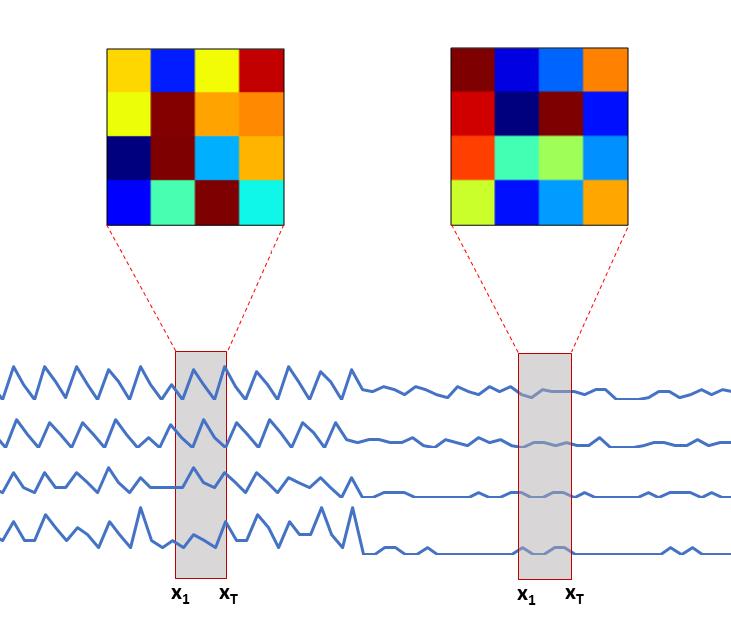
\includegraphics[width=0.8\linewidth]{fig1.png}
%\caption{Graph of $f(x)=ax^2|_{\{0.1, 0.3, 1.0, 3.0\}}$}
%\end{figure}

%----------------------------------------------------------------------------------------

\end{column} % End of the first column

\begin{column}{\sepwid}\end{column} % Empty spacer column

\begin{column}{\twocolwid} % Begin a column which is two columns wide (column 2)

\begin{figure}
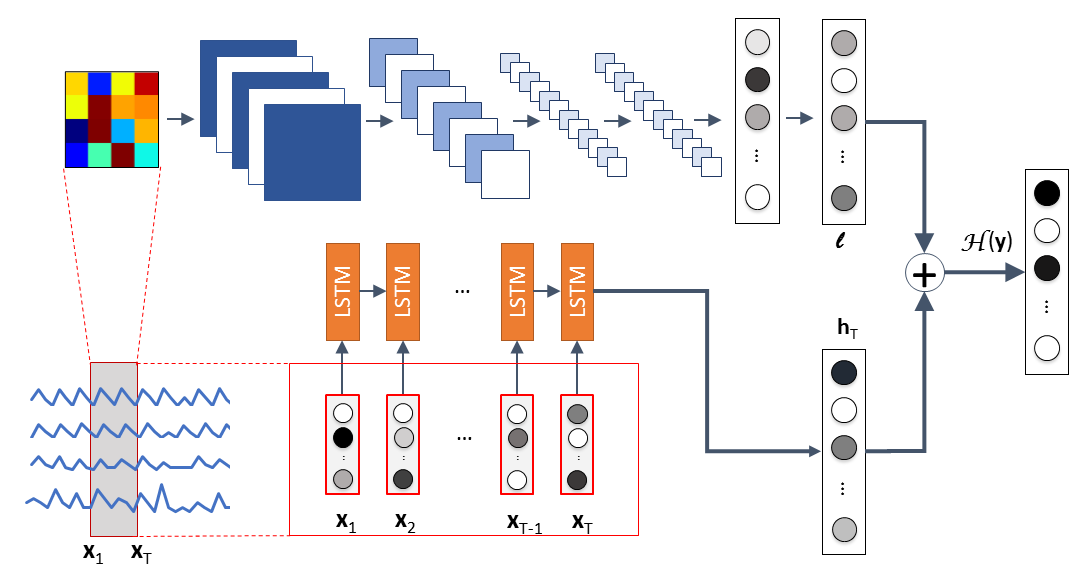
\includegraphics[width=0.8\linewidth]{fig2.png}
\caption{The network architecture for Deep $r$-RSJBE.}
\end{figure}

\begin{columns}[t,totalwidth=\twocolwid] % Split up the two columns wide column

\begin{column}{\onecolwid}\vspace{-.6in} % The first column within column 2 (column 2.1)

%----------------------------------------------------------------------------------------
%	MATERIALS
%----------------------------------------------------------------------------------------

\begin{block}{Binary Embedding}

\textbf{Raw time series representation}:
we aim to learn a mapping from 
$\bm{X}$ to $\bm{h}$  with
\vspace{2mm}
\begin{equation}\label{hp}
\bm{h}_{T} = \mathcal{F}(\mathbf{X}),
\vspace{2mm}
\end{equation}
where $\bm{h}\in \mathbb{R}^m$ is the feature vector, $m$ is the dimension of $\bm{h}$, and $\mathcal{F}$ denotes LSTM units.

\textbf{Correlation Map Representation}:
we construct a $n\times n$ correlation map based upon Pearson's correlation coefficient, \textit{i.e.},
\begin{equation}\label{hp}
\vspace{2mm}
c_{i}^{j}=\frac{\sum_{k=1}^{T}(x^i_k-\bar{x}^i)(x^j_k-\bar{x}^j)}{\sqrt{\sum_{k=1}^{T}(x^i_k-\bar{x}^i)^2\sum_{k=1}^{T}(x^j_k-\bar{x}^j)^2}}
\vspace{2mm}
\end{equation}
where $\bar{x}^i$ and $\bar{x}^j$ denotes sample means of the two time series.

As shown in Figure 1,  the CNNs in Deep $r$-RSJBE contain 4 convolutional layers (conv1-conv4 with $3\times 3\times 16$, $3\times 3\times 32$, $3\times 3\times 64$, and $3\times 3\times 64$ filters; as well as $1\times 1$, $2\times 2$, $2\times 2$, and $1\times 1$ strikes, respectively) and 2 fully connected layers (fc5-fc6). Each convolutional layer is followed by batch normalization and rectifier linear units (ReLU). Since $\bm{y}=[\bm{h}_T; \bm{l}]\in\mathbb{R}^{2m}$, the joint binary embedding is obtained by:
\begin{equation}\label{hash_fun}
\begin{aligned}
\mathcal{H}_c(\bm{y})=\mathrm{sgn}\big(\mathcal{F}_c(\bm{y})\big),\quad c=1,\cdots,v,
\end{aligned}
\end{equation}

\end{block}

%----------------------------------------------------------------------------------------

\end{column} % End of column 2.1

\begin{column}{\onecolwid}\vspace{-.6in} % The second column within column 2 (column 2.2)

%----------------------------------------------------------------------------------------
%	P
%----------------------------------------------------------------------------------------

\begin{block}{$r$-th Root Ranking Loss}


Given a set of triplets
$\mathcal{D}_{\rm{Triplet}}=\big\{(\mathbf{X}_{q}$, $\mathbf{X}_{i}$, $\mathbf{X}_{j})\big\}$,
in which the segment pair ($\mathbf{X}_{q}$, $\mathbf{X}_{i}$) is more similar than
the segment pair ($\mathbf{X}_{q}$, $\mathbf{X}_{j}$), then the ``rank" can be
defined as:
\begin{equation}\label{Rank}
\begin{aligned}
\mathrm{R}(\bm{y}_{q},\bm{y}_{i})=\sum_{j}\mathcal{I}\Big(
&\big\|\mathcal{H}(\bm{y}_{q})-\mathcal{H}(\bm{y}_{j})\big\|_{\mathrm{H}}
\le \big\|\mathcal{H}(\bm{y}_{q})-\mathcal{H}(\bm{y}_{i})\big\|_{\mathrm{H}}
\Big) \nonumber
\end{aligned}
\end{equation}
The $r$-th root ranking loss is defined as:
\begin{equation}\label{Loss}
\begin{aligned}
\mathcal{L}\big(\mathrm{R}(\bm{y}_{q},\bm{y}_{i})\big)=\mathrm{R}^{\frac{1}{r}}(\bm{y}_{q},\bm{y}_{i}),
\end{aligned}
\end{equation}
where $r>1$. This loss penalizes the segments that are incorrectly ranked at the top of a Hamming-distance ranking list
more than those at the bottom.

Therefore, the objective of Deep $r$-RSJBE is given by:
\begin{equation}\label{Obj}
\begin{aligned}
\mathcal
{O}(\mathcal{D}_{\rm{Triplet}},\mathbf{W})=\sum_{q}\sum_{i}\mathrm{R}^{\frac{1}{r}}(\bm{y}_{q},\bm{y}_{i})+\frac{\lambda}{2}\|\mathbf{W}\|_{\mathrm{F}}^{2}.
\end{aligned}
\end{equation}
\end{block}
\begin{figure}\vspace{-10mm}
     \begin{subfigure}[t]{0.4\textwidth}
            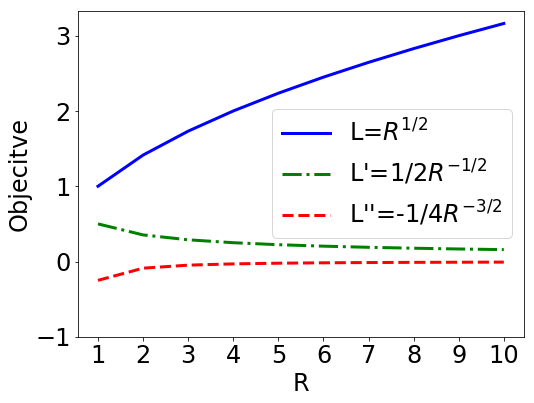
\includegraphics[width=\textwidth]{fig3a}
            \subcaption{}\label{fig:a}
     \end{subfigure}
     \quad
     \begin{subfigure}[t]{0.4\textwidth}
            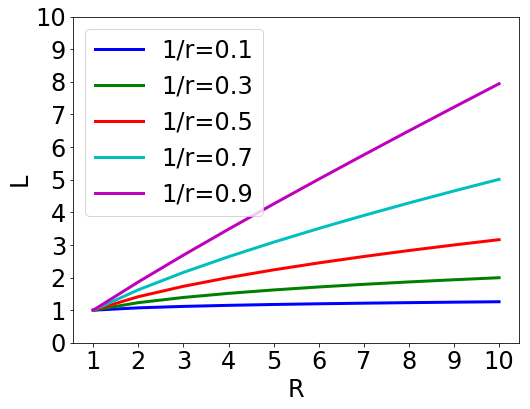
\includegraphics[width=\textwidth]{fig3b}
            \subcaption{}\label{fig:b}
     \end{subfigure}\vspace{-10mm}
      \caption{(a) Loss function $\mathcal{L}(R)$, its gradient $\mathcal{L}'(R)$, and $\mathcal{L}''(R)$ when $r=2$. (b) $\mathcal{L}(R)$ vs $r$ when $\frac{1}{r}=\{0.1,0.3,0.5,0.7,0.9\}$. }
 \end{figure}
%----------------------------------------------------------------------------------------

\end{column} % End of column 2.2

\end{columns} % End of the split of column 2 - any content after this will now take up 2 columns width

%----------------------------------------------------------------------------------------
%	IMPORTANT To REMEMBER
%----------------------------------------------------------------------------------------


%\begin{alertblock}{Myth of Delta $\Delta$}

%It's commonly believed that in order to work out roots of a quadratic function you must count $\Delta$ and use other previously established formulas. However this is untrue since factorising in many cases is as good or even better than simply counting $\Delta$.

%\end{alertblock} 

%----------------------------------------------------------------------------------------

\begin{columns}[t,totalwidth=\twocolwid] % Split up the two columns wide column again

\begin{column}{\onecolwid} % The first column within column 2 (column 2.1)

%----------------------------------------------------------------------------------------
%	EXAMPLE OF FACTORISATION
%----------------------------------------------------------------------------------------


%----------------------------------------------------------------------------------------

\end{column} % End of column 2.1

\begin{column}{\onecolwid} % The second column within column 2 (column 2.2)

%----------------------------------------------------------------------------------------
%	PROOF OF VIETA'S FORMULAS
%----------------------------------------------------------------------------------------

%----------------------------------------------------------------------------------------

\end{column} % End of column 2.2

\end{columns} % End of the split of column 2

\end{column} % End of the second column

\begin{column}{\sepwid}\end{column} % Empty spacer column

\begin{column}{\onecolwid} % The third column

%----------------------------------------------------------------------------------------
%	CONCLUSION
%----------------------------------------------------------------------------------------

\begin{block}{Experiment}

\begin{table}\scriptsize
\vspace{-20mm}
\centering \caption{Multivariate time series retrieval performance (\textbf{MAP}) on EEG Eye State and PAMAP2
 when $v=32$, $64$, $128$.} \label{tab:table2} \vspace{-3mm} \centering {
\vspace{3mm}\begin{tabular}{|c|c|c|c|c|c|c|c|} \hline
 \multicolumn{1}{|c|}{\textbf{Algorithms}}&\multicolumn{3}{c|}{\textbf{EEG Eye State} }&\multicolumn{3}{c|}{\textbf{PAMAP2} } \\ \hline
$\sharp$ \textbf{Bits}                       & $v=$32  & $v=$64  & $v=$128   & $v=32$ & $v=64$  & $v=128$ \\
\hline\hline
LSH    &  0.5326  & 0.5335   & 0.5355   & 0.3354  &  0.3684  & 0.4030   \\
\hline
ITQ       &  0.5435  & 0.5425  & 0.5439     & 0.3870 &  0.3849  & 0.4087     \\
\hline\hline

HDML   &   0.5646  & 0.5716  &  0.5714  &  0.5552 &  0.5919 & 0.6191   \\
\hline
TopRSBC       &   0.5803 &  0.5832 & 0.5876    &  0.5758  &   0.6036  &    0.6149   \\

\hline\hline
CNNs+Pairwise loss   &   0.9567  & 0.9551  &  0.9569  &  0.6416  &  0.6327 & 0.6261 \\
\hline
LSTM+Triplet loss       &   0.9570 &  0.9464 & 0.9433   & 0.6409 &  0.6662 & 0.6280    \\

\hline\hline  
LSTM+$r$-th root ranking loss             &  0.9805  &  0.9849 &   0.9663 & 0.6588  &  0.6779 & 0.6506 \\ \hline
Deep $r$-RSJBE &  \textbf{0.9869} &
\textbf{0.9855}  &   \textbf{0.9796} & \textbf{0.8381}  & \textbf{0.8102} & \textbf{0.7948} 
\\
\hline

\end{tabular}
 \vspace{-2mm}
       }
\end{table}

\begin{figure}\vspace{2mm}
     \begin{subfigure}[t]{0.45\textwidth}
            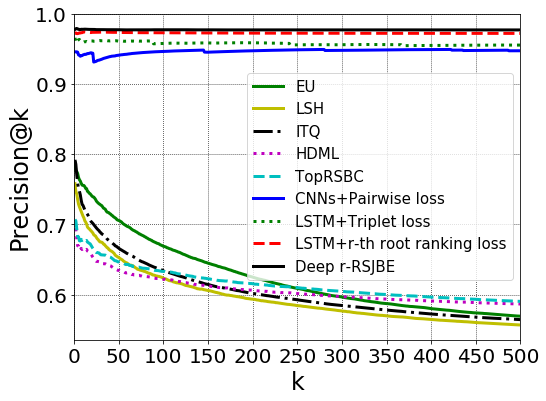
\includegraphics[width=\textwidth]{fig4a}
            \subcaption{Precision@k}\label{fig:a}
     \end{subfigure}
     \quad
     \begin{subfigure}[t]{0.45\textwidth}
            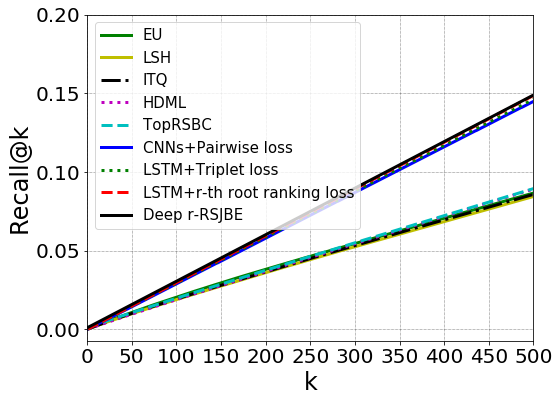
\includegraphics[width=\textwidth]{fig5a}
            \subcaption{Recall@k}\label{fig:b}
     \end{subfigure}
      \caption{Precision@k and Recall@k with 32 binary bits on EEG Eye State.}\vspace{-5mm}
 \end{figure}
 
 \begin{figure}\vspace{2mm}
     \begin{subfigure}[t]{0.45\textwidth}
            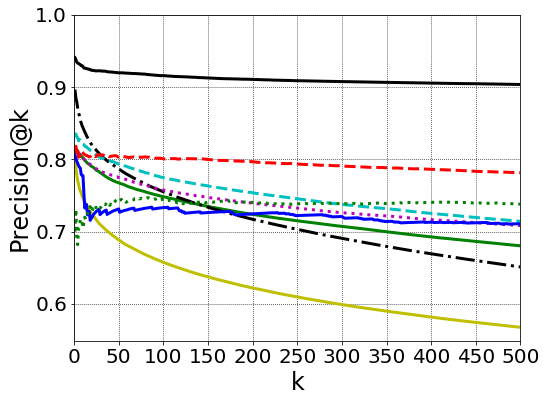
\includegraphics[width=\textwidth]{fig4b}
            \subcaption{Precision@k}\label{fig:a}
     \end{subfigure}
     \quad
     \begin{subfigure}[t]{0.45\textwidth}
            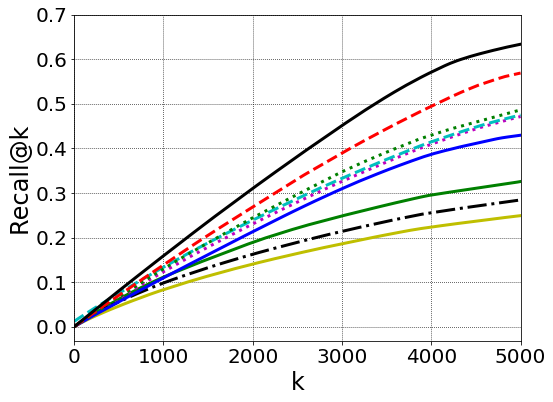
\includegraphics[width=\textwidth]{fig5b}
            \subcaption{Recall@k}\label{fig:b}
     \end{subfigure}
      \caption{Precision@k and Recall@k with 32 binary bits on PAMAP2.}\vspace{-5mm}
 \end{figure}
  \vspace{-5mm}
% \begin{figure}\vspace{2mm}
%     \begin{subfigure}[t]{0.45\textwidth}
%            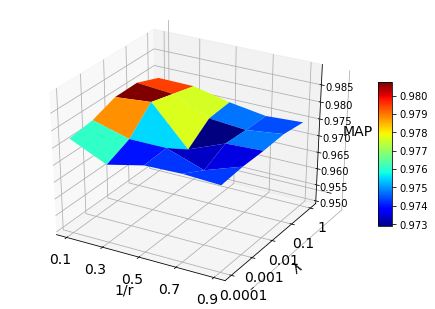
\includegraphics[width=\textwidth]{fig_ps_a}
%            \subcaption{EEG Eye State}\label{fig:a}
%     \end{subfigure}
%     \quad
%     \begin{subfigure}[t]{0.45\textwidth}
%            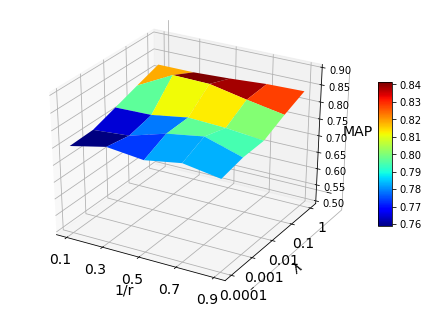
\includegraphics[width=\textwidth]{fig_ps_b}
%            \subcaption{PAMAP2}\label{fig:b}
%     \end{subfigure}
%      \caption{The parameter sensitivity of Deep $r$-RSJBE with respect to $\lambda = \{0.0001, 0.001, 0.01, 0.1, 1\}$ and $\frac{1}{r}=\{0.1, 0.3, 0.5, 0.7,$ $ 0.9\}$ when $v=32$ bits.. }\vspace{-5mm}
% \end{figure}
 \vspace{-10mm}
  \begin{table} \scriptsize
  \caption{The efficiency of Deep $r$-RSJBE on two datasets ($v$=32 bits).}
  \label{tab:freq}
  \begin{tabular}{|c|c|c|c|}
    \hline
    Dataset & training time & binary embedding & query time\\
    \hline \hline
    EEG Eye State & 238.41 &  1.72$\times10^{-5}$ &  5.05$\times10^{-4}$ \\ \hline
    PAMAP2  & 4842.54 & 1.46$\times10^{-5}$ &  2.60$\times10^{-3}$ \\ \hline
 %   SHL & 4814.40 & 1.61$\times10^{-5}$ & 7.92$\times10^{-3}$\\ \hline
\end{tabular}
\end{table}
 \vspace{-10mm}
\end{block}


%----------------------------------------------------------------------------------------
%	ACKNOWLEDGEMENTS
%----------------------------------------------------------------------------------------



\begin{alertblock}{Conclusion}

We developed a Deep $r$-th root of Rank Supervised Joint Binary Embedding (Deep $r$-RSJBE) to perform multivariate time series retrieval. 
Our empirical studies demonstrated the effectiveness and the efficiency of the proposed Deep $r$-RSJBE.
\end{alertblock}\vspace{-10mm}
\textbf{Contact information}: dsong@nec-labs.com
%----------------------------------------------------------------------------------------

\end{column} % End of the third column

\end{columns} % End of all the columns in the poster

\end{frame} % End of the enclosing frame

\end{document}
